%%%%%%%%%%%%%%%%%%%%%%%%%%%%%%%%%%%%%%
  %%%%%%%%%%%%%%%%%%%%%%%%%%%%%%%%%%%%%%
  % Do not edit the TeX file your work
% will be overwritten.  Edit the RnW
% file instead.
%%%%%%%%%%%%%%%%%%%%%%%%%%%%%%%%%%%%%%
  %%%%%%%%%%%%%%%%%%%%%%%%%%%%%%%%%%%%%%
  
  
      



\begin{knitrout}
\definecolor{shadecolor}{rgb}{0.969, 0.969, 0.969}\color{fgcolor}\begin{figure}[!h]

{\centering 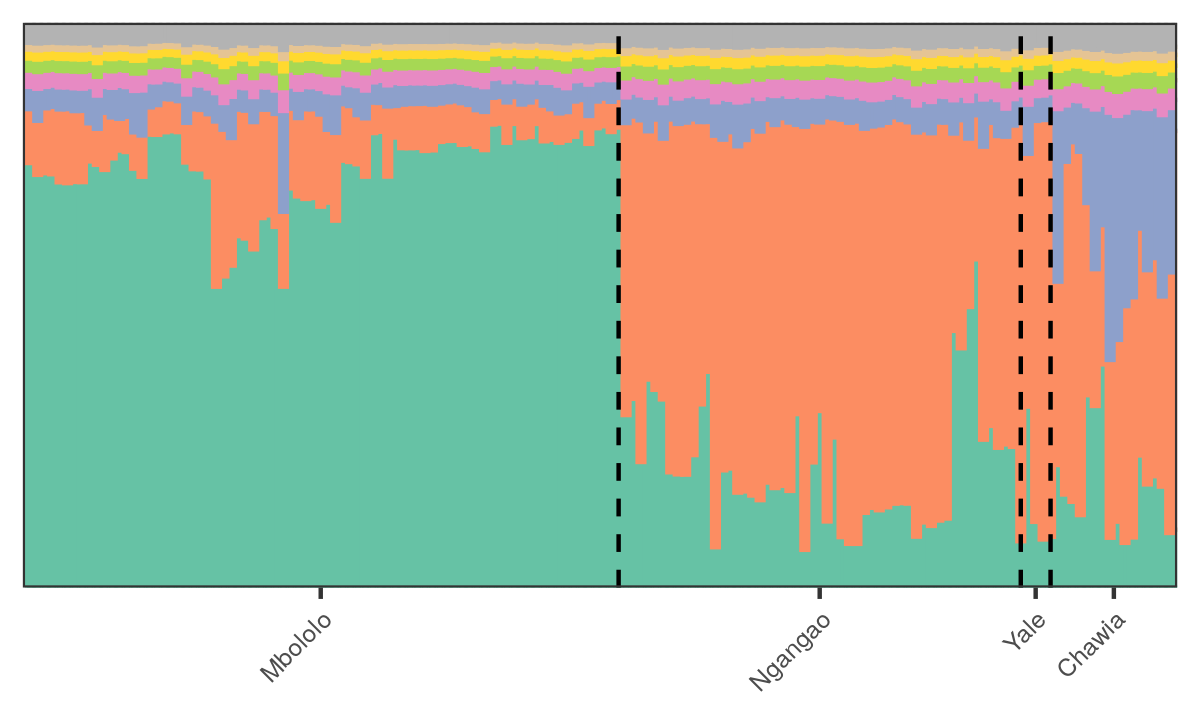
\includegraphics[width=0.980\linewidth,height=0.588\linewidth]{figure/stru_init_fit-1} 

}

\caption[The inferred individual admixtures at $\alpha = 3$]{The inferred individual admixtures at $\alpha = 3$. 
    Each vertical strip is an individual and each color
    an ancestral population.
    Lengths of colored segments represent the inferred mixture proportions.
    Mbololo, Ngangao, Yale, and Chawia refer to
    geographic regions from which each individual was collected. }\label{fig:stru_init_fit}
\end{figure}


\end{knitrout}

    
    

\begin{knitrout}
\definecolor{shadecolor}{rgb}{0.969, 0.969, 0.969}\color{fgcolor}\begin{figure}[!h]

{\centering 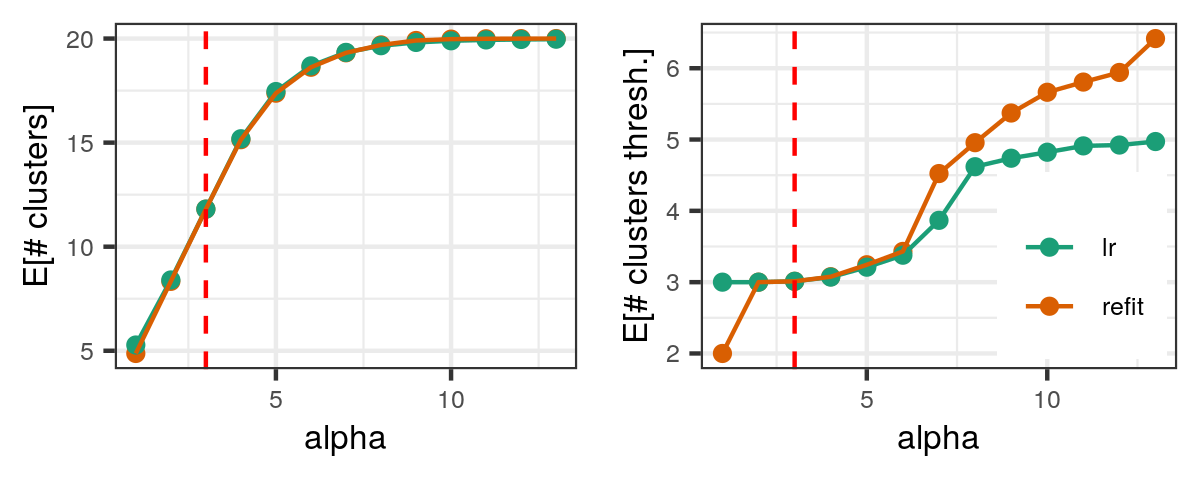
\includegraphics[width=0.980\linewidth,height=0.392\linewidth]{figure/stru_alpha_nclusters-1} 

}

\caption[The expected number of clusters in the thrush data as $\alpha$ varies.
    We compute the linear approximation at $\alpha = 3$]{The expected number of clusters in the thrush data as $\alpha$ varies.
    We compute the linear approximation at $\alpha = 3$. In the right plot, the threshold is set at $t = 20$ (approximately $1\%$ of loci). }\label{fig:stru_alpha_nclusters}
\end{figure}


\end{knitrout}




\begin{knitrout}
\definecolor{shadecolor}{rgb}{0.969, 0.969, 0.969}\color{fgcolor}\begin{figure}[!h]

{\centering 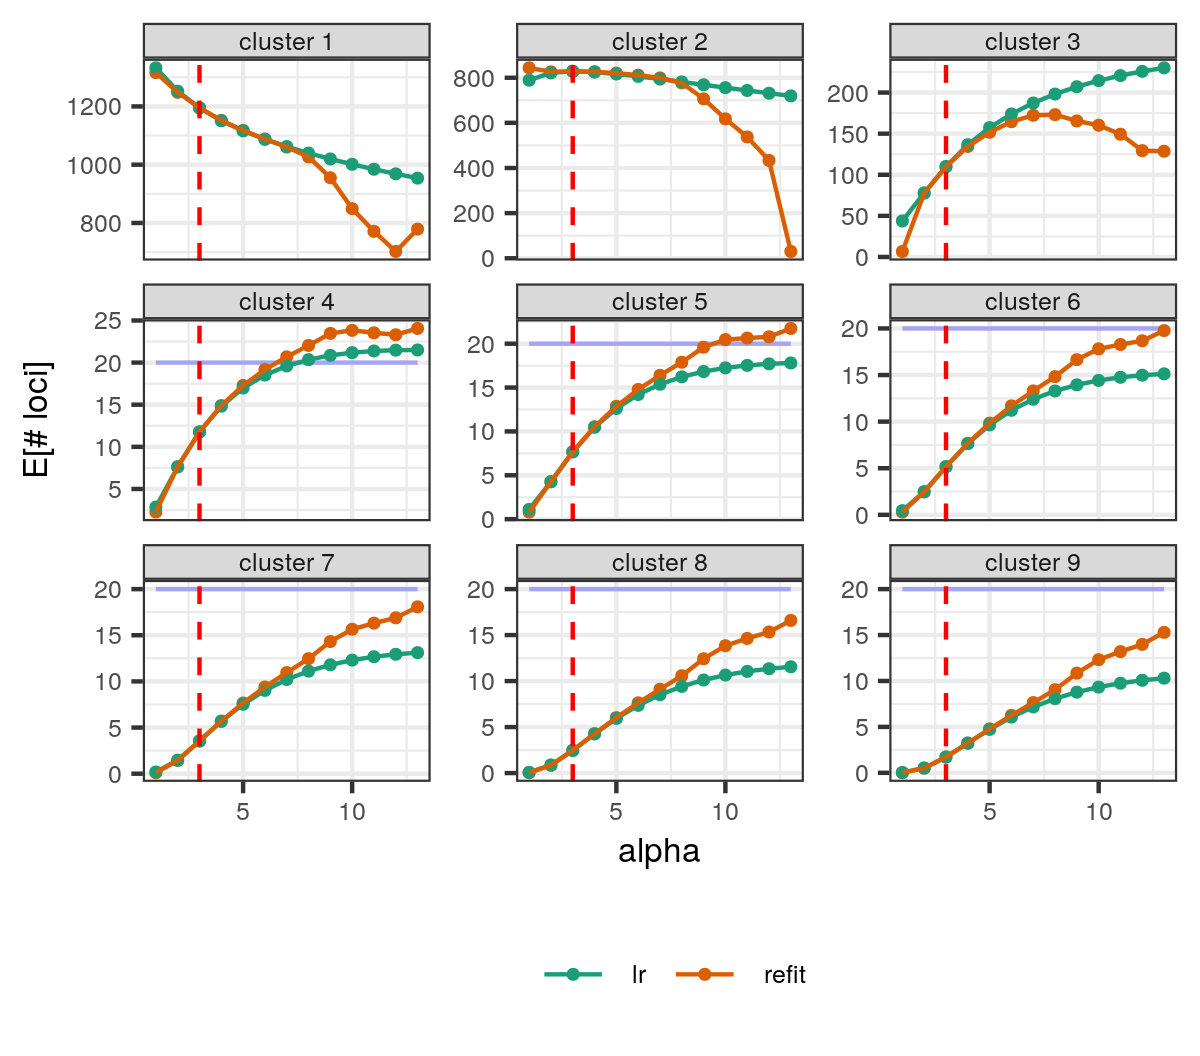
\includegraphics[width=0.980\linewidth,height=0.862\linewidth]{figure/stru_alpha_cluster_weights-1} 

}

\caption{The expected number of loci per cluster as $\alpha$ varies. 
     We compute the linear approximation at $\alpha = 3$. 
     The horizontal blue line corresponds to the threshold in computing the 
    expected number of thresholded clusters in Figure~\ref{fig:stru_alpha_nclusters} }\label{fig:stru_alpha_cluster_weights}
\end{figure}


\end{knitrout}



\begin{knitrout}
\definecolor{shadecolor}{rgb}{0.969, 0.969, 0.969}\color{fgcolor}\begin{figure}[!h]

{\centering 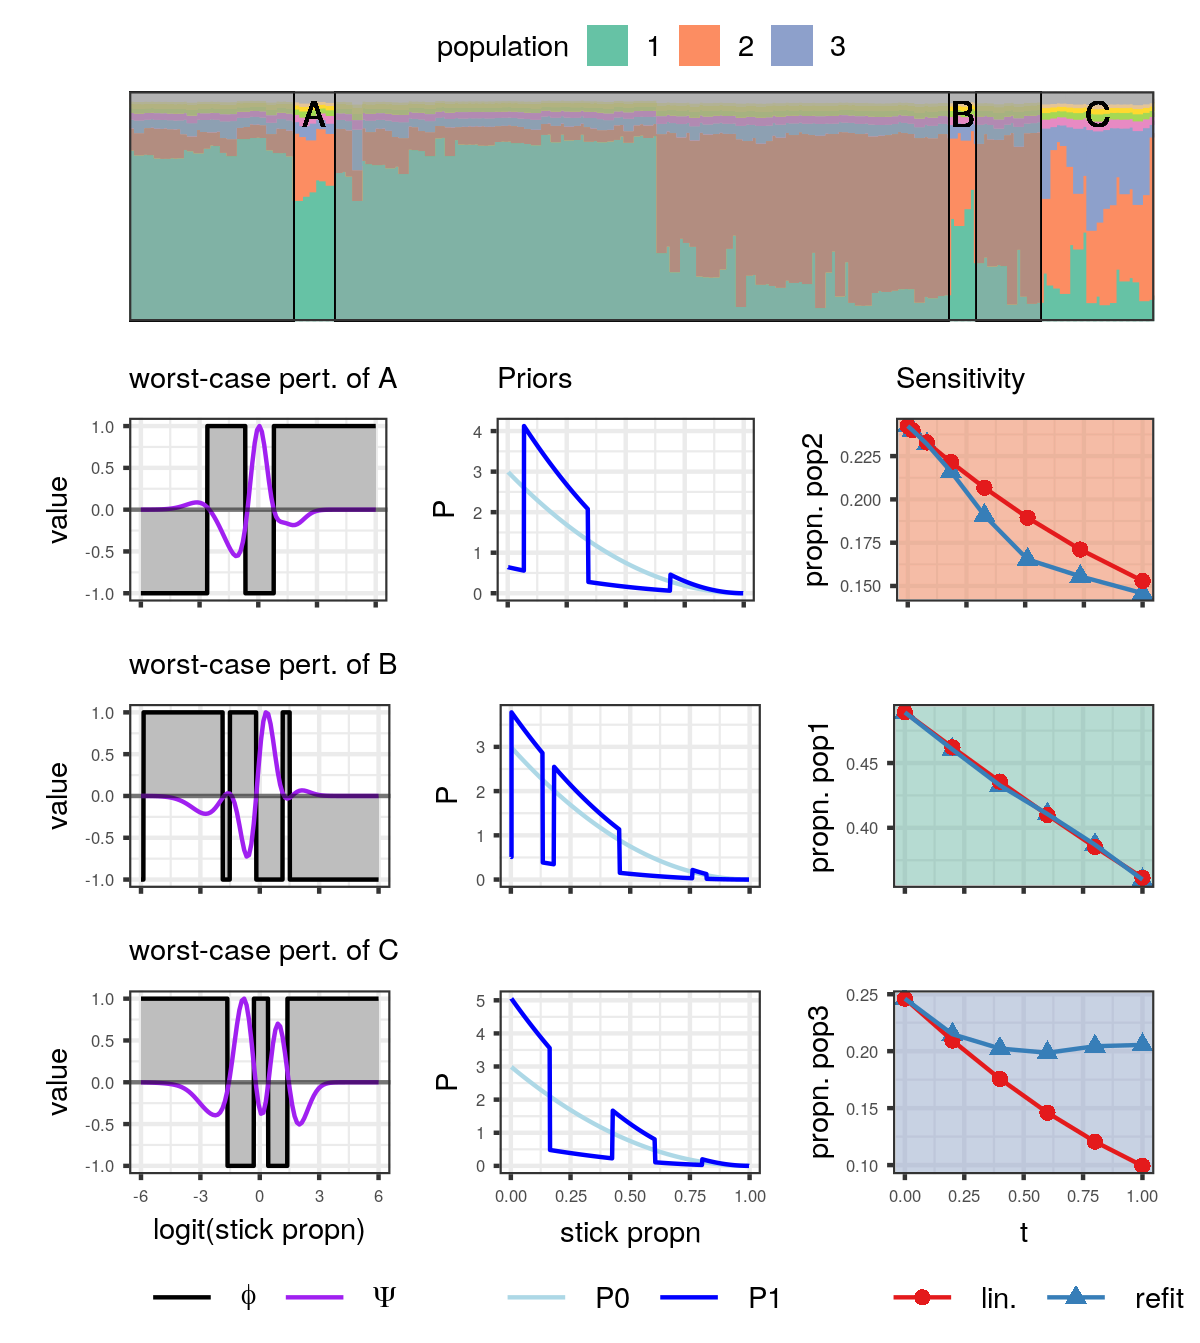
\includegraphics[width=0.980\linewidth,height=1.098\linewidth]{figure/stru_func_sens-1} 

}

\caption[Sensitivity of inferred admixtures for several outlying individuals]{Sensitivity of inferred admixtures for several outlying individuals. 
     For individuals A, 
     we examine the sensitivity of the inferred mixture proportion of the orange
     population.
     For individuals B, 
     we examine the inferred green proportion.
     For the individuals C, we examine the inferred purple proportion.
     (Left column) The worst-case $L_\infty$ negative perturbation in grey,
     plotted against the prior-weighted influence function
     (scaled to have $L_\infty$ norm equal to 1). 
    (Middle column) The effect of this perturbation on the prior density. 
    (Right column) Effects on the inferred admixture. }\label{fig:stru_func_sens}
\end{figure}


\end{knitrout}


\begin{knitrout}
\definecolor{shadecolor}{rgb}{0.969, 0.969, 0.969}\color{fgcolor}\begin{figure}[!h]

{\centering 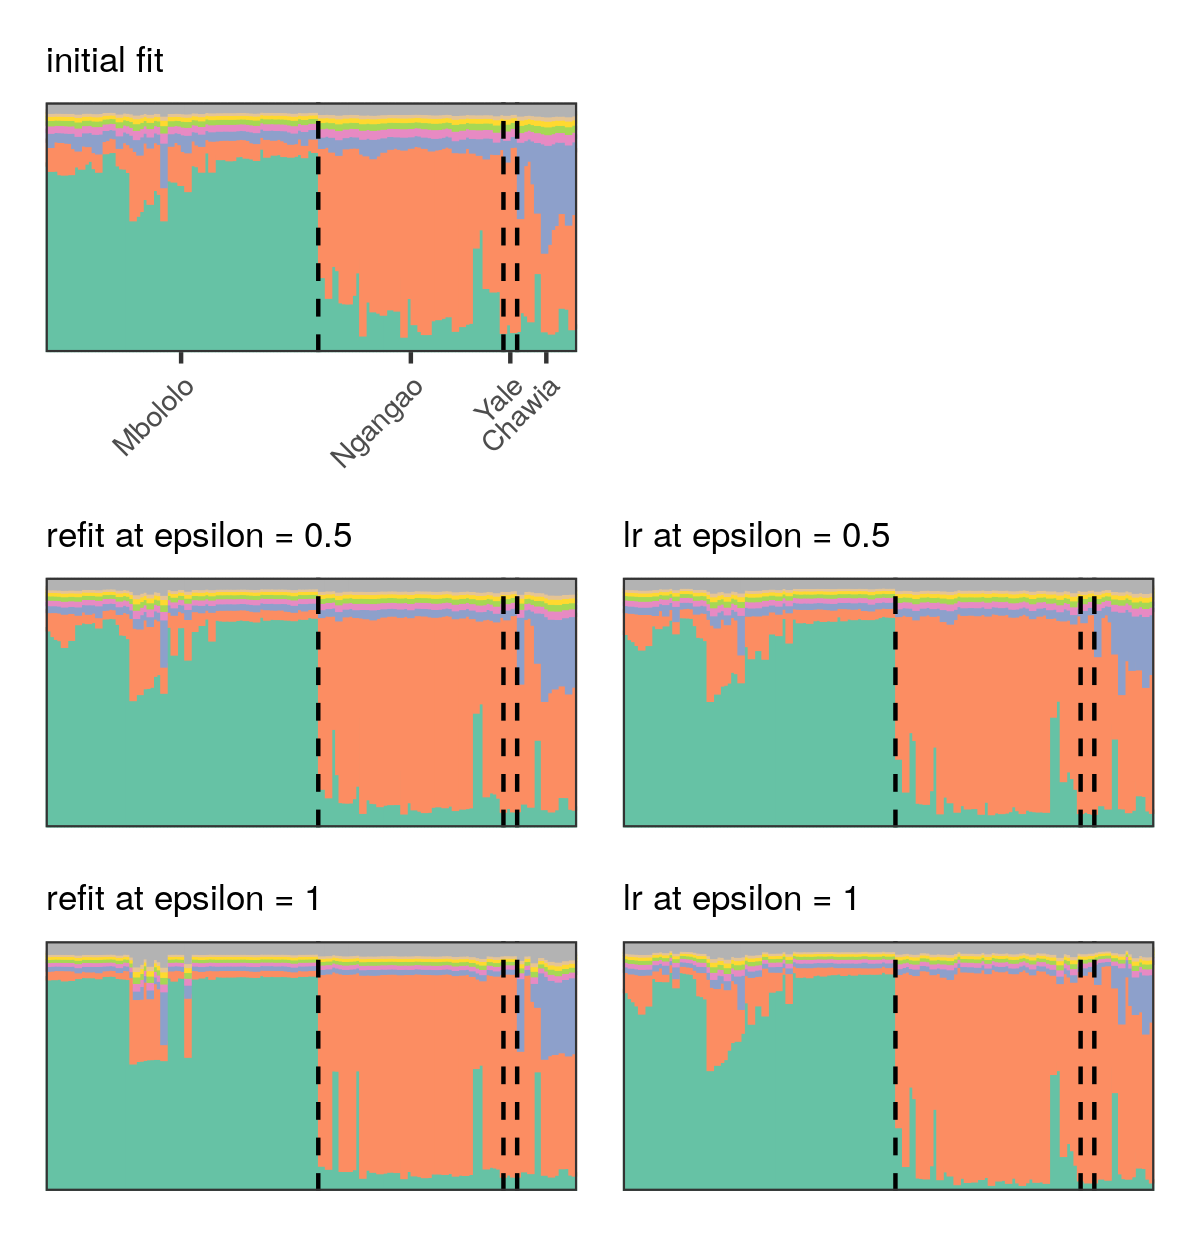
\includegraphics[width=0.980\linewidth,height=1.019\linewidth]{figure/stru_func_sens_admix-1} 

}

\caption{Inferred admixtures after the worst-case prior perturbation 
     to individuals A (second row, Figure~\ref{fig:stru_func_sens}). }\label{fig:stru_func_sens_admix}
\end{figure}


\end{knitrout}


